%--------------------------------------------------------------------------------------------------%
%	The MIT License (MIT)
%
%	Copyright (c) 2015 Jan Küster
%
%	Permission is hereby granted, free of charge, to any person obtaining a copy
%	of this software and associated documentation files (the "Software"), to deal
%	in the Software without restriction, including without limitation the rights
%	to use, copy, modify, merge, publish, distribute, sublicense, and/or sell
%	copies of the Software, and to permit persons to whom the Software is
%	furnished to do so, subject to the following conditions:
%
%	THE SOFTWARE IS PROVIDED "AS IS", WITHOUT WARRANTY OF ANY KIND, EXPRESS OR
%	IMPLIED, INCLUDING BUT NOT LIMITED TO THE WARRANTIES OF MERCHANTABILITY,
%	FITNESS FOR A PARTICULAR PURPOSE AND NONINFRINGEMENT. IN NO EVENT SHALL THE
%	AUTHORS OR COPYRIGHT HOLDERS BE LIABLE FOR ANY CLAIM, DAMAGES OR OTHER
%	LIABILITY, WHETHER IN AN ACTION OF CONTRACT, TORT OR OTHERWISE, ARISING FROM,
%	OUT OF OR IN CONNECTION WITH THE SOFTWARE OR THE USE OR OTHER DEALINGS IN
%	THE SOFTWARE.
%
%
%--------------------------------------------------------------------------------------------------%


%============================================================================
%
%	DOCUMENT DEFINITION
%
%============================================================================

% Use article class to fully customize the page (do not use use a CV template)
\documentclass[10pt,x11names]{article}

\usepackage[utf8]{inputenc}

\usepackage{xifthen}  % provides \isempty test

%----------------------------------------------------------------------------------------
%	FONT
%----------------------------------------------------------------------------------------

% some tex-live fonts - choose your own

%\usepackage[defaultsans]{droidsans}
%\usepackage[default]{comfortaa}
%\usepackage{cmbright}
%\usepackage[default]{raleway}
%\usepackage{fetamont}
\usepackage[default]{gillius}
%\usepackage[light,math]{iwona}
%\usepackage[thin]{roboto}

% set font default
\renewcommand*\familydefault{\sfdefault}

\usepackage{moresize}     % more font size definitions
\usepackage{fontawesome}
\usepackage{emoji}
\usepackage{tabularx}

%----------------------------------------------------------------------------------------
%	PAGE LAYOUT  DEFINITIONS
%----------------------------------------------------------------------------------------

%debug page outer frames
%\usepackage{showframe}

% define page size and styles using geometry
\usepackage[paperheight=297mm, paperwidth=210mm]{geometry} % [a4paper] [heightrounded]???

% for example, change the margins to 2 inches all round
\geometry{top=0.8cm, bottom=-.6cm, left=0.4cm, right=1cm}

% less space between header and content
\setlength{\headheight}{-5pt}

%indentation is zero
\setlength{\parindent}{0mm}

%----------------------------------------------------------------------------------------
%	TABLE /ARRAY DEFINITIONS
%----------------------------------------------------------------------------------------

% Layouting tables
\usepackage{multicol}
\usepackage{multirow}

% Extended aligning of tabular cells
\usepackage{array}

\newcolumntype{x}[1]{%
>{\raggedleft\hspace{0pt}}p{#1}}%

%----------------------------------------------------------------------------------------
%	GRAPHICS DEFINITIONS
%----------------------------------------------------------------------------------------

\usepackage{graphicx}

% For floating figures
\usepackage{wrapfig}
\usepackage{float}
%\floatstyle{boxed}
%\restylefloat{figure}

% For drawing graphics
\usepackage{tikz}
\usetikzlibrary{shapes, backgrounds,mindmap, trees}

% Bubble diagrams
\usepackage{smartdiagram}
\smartdiagramset{
    bubble center node font = \footnotesize,
    bubble node font = \footnotesize,
    % specifies the minimum size of the bubble center node
    bubble center node size = 0.5cm,
    %  specifies the minimum size of the bubbles
    bubble node size = 0.9cm,
    % specifies which is the distance among the bubble center node and the other bubbles
    distance center/other bubbles = 0.5cm,
%     % sets the distance from the text to the border of the bubble center node
%     distance text center bubble = 0.5cm,
%     % set center bubble color
%     bubble center node color = pastelblue,
%     % define the list of colors usable in the diagram
%     set color list = {lightgray, materialcyan, orange, green, materialorange, materialteal, materialamber, materialindigo, materialgreen, materiallime},
%     % sets the opacity at which the bubbles are shown
%     bubble fill opacity = 0.6,
%     % sets the opacity at which the bubble text is shown
%     bubble text opacity = 1,
}

%----------------------------------------------------------------------------------------
%	Color DEFINITIONS
%----------------------------------------------------------------------------------------

\usepackage{transparent}
\usepackage{xcolor}

% Accent color
\definecolor{complcol}{RGB}{250,150,10}

% Light background
\definecolor{softcol}{RGB}{225,225,225}

% Custom colors
\definecolor{pastelblue}{HTML}{0395DE}
\definecolor{customblue1}{HTML}{428bca}

\definecolor{scala2blue}{HTML}{e45c77}
\definecolor{scala3rose}{HTML}{5cc6e4}
% From the \lambda Haskell logo (L to R): 453a62 5e5086 8f4e8b <- purples,  3f3f3f <- gray
\definecolor{haskell1}{HTML}{453a62}
\definecolor{haskell2}{HTML}{5e5086}
\definecolor{haskell3}{HTML}{8f4e8b}
\definecolor{haskell4}{HTML}{3f3f3f}

\definecolor{haskellweb1}{HTML}{3d1f54}
\definecolor{haskell2custom1}{HTML}{5a4b82}
\definecolor{haskell2custom2}{HTML}{5b4796}

% --vvv-- Color schemes --vvv--

% Bright brown/blue
% \colorlet{bgcol}{Sienna3}
% \colorlet{sectcol}{DodgerBlue1}
% \colorlet{sidecolor}{DodgerBlue3}
% \colorlet{introcolor}{bgcol}

% Pale gray/blue
% \colorlet{bgcol}{Ivory4}
% \colorlet{sectcol}{customblue1}
% \colorlet{sidecolor}{sectcol}
% \colorlet{introcolor}{bgcol}

% Scala2/3 schema (like)
% \colorlet{bgcol}{scala3rose}
% \colorlet{sectcol}{scala2blue}
% \colorlet{sidecolor}{scala2blue}
% \colorlet{introcolor}{bgcol}

% Haskell schema
\colorlet{bgcol}{haskellweb1}
\colorlet{sectcol}{haskell2custom1}
\colorlet{sidecolor}{haskell4}
\colorlet{introcolor}{haskell3}

% Package for links, must be the last package used
\usepackage[
  colorlinks = true,
%   linkcolor = blue,
%   urlcolor = blue,
%   citecolor = blue,
%   anchorcolor = blue,
]{hyperref}

%============================================================================%
%
%
%	DEFINITIONS
%
%
%============================================================================%

% Returns minipage width minus two times \fboxsep
% to keep padding included in width calculations
\newcommand{\mpwidth}{\linewidth-\fboxsep-\fboxsep}

%----------------------------------------------------------------------------------------
% 	ARROW GRAPHICS in Tikz
%----------------------------------------------------------------------------------------

% a six pointed arrow poiting to the left
\newcommand{\tzlarrow}{(0,0) -- (0.2,0) -- (0.3,0.2) -- (0.2,0.4) -- (0,0.4) -- (0.1,0.2) -- cycle;}

% include the left arrow into a tikz picture
% param1: fill color
%
\newcommand{\larrow}[1]
{\begin{tikzpicture}[scale=0.58]
	 \filldraw[fill=#1!100,draw=#1!100!black]  \tzlarrow
 \end{tikzpicture}
}

% a six pointed arrow pointing to the right
\newcommand{\tzrarrow}{ (0,0.2) -- (0.1,0) -- (0.3,0) -- (0.2,0.2) -- (0.3,0.4) -- (0.1,0.4) -- cycle;}

% include the right arrow into a tikz picture
% param1: fill color
%
\newcommand{\rarrow}
{\begin{tikzpicture}[scale=0.7]
	\filldraw[fill=sectcol!100,draw=sectcol!100!black] \tzrarrow
 \end{tikzpicture}
}

%----------------------------------------------------------------------------------------
%	custom sections
%----------------------------------------------------------------------------------------

% create a coloured box with arrow and title as cv section headline
% param 1: section title
%
\newcommand{\cvsection}[1]{
  \colorbox{sectcol}{\mystrut \makebox[1\mpwidth][l]{
  \larrow{introcolor!70!white} \hspace{-8pt} \larrow{introcolor!40!white} \hspace{-8pt} \larrow{introcolor!10!white} \textbf{\textcolor{white}{\uppercase{#1}}}\hspace{4pt}
  }}\\
}

% create a coloured arrow with title as cv meta section section
% param 1: meta section title
%
\newenvironment{metasection}[1] {
	\vspace{6pt}
	\begin{center}
		\textcolor{white}{\large{\uppercase{#1}}}\\
	\normalsize
	\parbox{0.7\mpwidth}{\textcolor{white}	\hrule}
}{\end{center}}

%----------------------------------------------------------------------------------------
%	 CV ENTRIES: cvposition, cventry, cvevent (the original one)
%----------------------------------------------------------------------------------------

% Company/position heading command
% arg1: dates
% arg2: position
% arg3: company
\newcommand{\cvposition}[3]{
  \begin{tabular*}{1\mpwidth}{p{0.45\mpwidth}  x{0.52\mpwidth}}
    \textcolor{black}{\textbf{#2}} & \textcolor{complcol}{#3}, \textcolor{gray}{#1}
  \end{tabular*}
  \textcolor{softcol}{\hrule}
  \vspace{6pt}
}

\newcommand{\cventry}[1]{
  \begin{minipage}[t]{0.04\mpwidth}
    \hspace{3pt}\larrow{softcol}
  \end{minipage}
  \begin{minipage}[t]{0.97\mpwidth}
    #1\\[-5pt]
  \end{minipage}
  %\par
  %\vspace{5pt}
}

% creates a stretched box as cv entry headline followed by two paragraphs about
% the work you did
% param 1:	event time i.e. 2014 or 2011-2014 etc.
% param 2:	event name (what did you do?)
% param 3:	institution (where did you work / study)
% param 4:	what was your position
% param 5:	some words about your contributions
%
\newcommand{\cvevent}[5]
{
\vspace{8pt}
	\begin{tabular*}{1\mpwidth}{p{0.55\mpwidth}  x{0.42\mpwidth}}
 	\textcolor{black}{\textbf{#2}} & \textcolor{complcol}{#3}, \textcolor{bgcol}{#1}

	\end{tabular*}
\vspace{-12pt}
\textcolor{softcol}{\hrule}
\vspace{6pt}
	\begin{tabular*}{0.5\mpwidth}{p{\mpwidth}}
\larrow{softcol}  #4\\[3pt]
\larrow{softcol}  #5\\[6pt]
	\end{tabular*}
}

% creates a stretched box as
\newcommand{\cveventmeta}[2]
{
	\mbox{\mystrut \hspace{87pt}\textit{#1}}\\
	#2
}

%----------------------------------------------------------------------------------------
% CUSTOM STRUT FOR EMPTY BOXES
%----------------------------------------- -----------------------------------------------
\newcommand{\mystrut}{\rule[-.3\baselineskip]{0pt}{\baselineskip}}

%----------------------------------------------------------------------------------------
% CUSTOM LOREM IPSUM
%----------------------------------------------------------------------------------------
\newcommand{\lorem}
{Lorem ipsum dolor sit amet, consectetur adipiscing elit. Donec a diam lectus.}

% use to vertically center content
% credits to: http://tex.stackexchange.com/questions/7219/how-to-vertically-center-two-images-next-to-each-other
\newcommand{\vcenteredinclude}[1]{\begingroup
\setbox0=\hbox{\includegraphics{#1}}%
\parbox{\wd0}{\box0}\endgroup}

% use to vertically center content
% credits to: http://tex.stackexchange.com/questions/7219/how-to-vertically-center-two-images-next-to-each-other
\newcommand*{\vcenteredhbox}[1]{\begingroup
\setbox0=\hbox{#1}\parbox{\wd0}{\box0}\endgroup}

%----------------------------------------------------------------------------------------
%	ICON MACROS
%----------------------------------------------------------------------------------------

% args: (iconName, boxSize, color)
\newcommand{\icon}[3]{%	                        %icon shortcut
    \vcenteredhbox{\makebox(#2, #2){\textcolor{#3}{\csname fa#1\endcsname}}}%
}

% args: (iconName, boxSize, text, color)
\newcommand{\icontext}[4]{ 						%icon with text shortcut
    \vcenteredhbox{\icon{#1}{#2}{#4}} \vcenteredhbox{\textcolor{#4}{#3}}
}

% args: (iconName, boxSize, text, url, textColor)
\newcommand{\iconhref}[5]{ 						%icon with website url
    \vcenteredhbox{\icon{#1}{#2}{#5}} \href{#4}{\textcolor{#5}{#3}}
}

% args: (iconName, boxSize, text, mailto, color)
\newcommand{\iconemail}[5]{ 					%icon with email link
    \vcenteredhbox{\icon{#1}{#2}{#5}} \href{mailto:#4}{\textcolor{#5}{#3}}
}

%----------------------------------------------------------------------------------
%  Fork me on GitHub
%----------------------------------------------------------------------------------

\usepackage{tikz}
\usepackage{ifthen}
\usepackage{xcolor}
\usetikzlibrary{shadows.blur}

\definecolor{forkmebg}{HTML}{3873b3}
\definecolor{forkmefg}{HTML}{eeeeee}

% rotate and shift are hardcoded here because of the href workaround, see also https://gist.github.com/dokenzy/fe8967c8a5921191a261
\newcommand{\forkme}{
  \begin{tikzpicture}[remember picture, overlay]
    \node[rotate=-50, shift={(-1.7cm, -1.7cm)}] at (current page.north east) {
      \begin{tikzpicture}[remember picture, overlay]
        \node[fill=forkmebg, text centered, minimum width=50em, minimum height=2.3em, blur shadow, shadow yshift=0pt, shadow xshift=0pt, shadow blur radius=.4em, shadow opacity=50](fmogh) at (0pt, 0pt) {}; % workaround: text/link see below
        \draw[forkmefg!60, dashed, line width=.08em, dash pattern=on .5em off 1.5\pgflinewidth] (-25em,0.9em) rectangle (25em,-0.9em);
      \end{tikzpicture}
    };
    % workaround: the link needs to be defined using a \rotatebox{deg} because \node[rotate=deg]{\href} isn't rendered correctly
    \node[shift={(-1.10cm, -1.35cm)}, text centered, minimum width=50em, minimum height=3.0em, text=forkmefg](fmogh) at (current page.north east) {\fontfamily{phv}\selectfont\bfseries \href{https://github.com/gerardbosch/resume}{\rotatebox{-50}{\color{white}{\small Fork me on GitHub}}} };
  \end{tikzpicture}
}

%============================================================================
%
%	DOCUMENT CONTENT
%
%============================================================================

\begin{document}
\fcolorbox{white}{white}{\begin{minipage}[b][0.966\textheight][t]{0.69\linewidth}


%---------------------------------------------------------------------------------------
%	TITLE HEADLINE
%----------------------------------------------------------------------------------------

\vspace{-3pt}
\colorbox{bgcol}{\color{white}\makebox[\mpwidth][c]{
  \hspace{46pt}\HUGE{\uppercase{Gerard Bosch} }
  \textcolor{introcolor}{\rule[-1mm]{1mm}{0.9cm}}
  \parbox[b]{5cm}{
    \large{{Software Engineer}} \\
    \large{{Craftsman}}
  }
}}

% Live resume note
\vspace{1pt}\centerline{
  \href{https://resume.gerardbosch.xyz}{\emoji{person-gesturing-ok} \textcolor{black}{This \emph{résumé} is \textcolor{magenta}{live!} Click here to ensure you access the most \textbf{up-to-date} version \emoji{person-gesturing-ok}}}
}\vspace{1pt}


%----------------------------------------------------------------------------------------
%	HEADER IMAGE / BANNER
%----------------------------------------------------------------------------------------

% 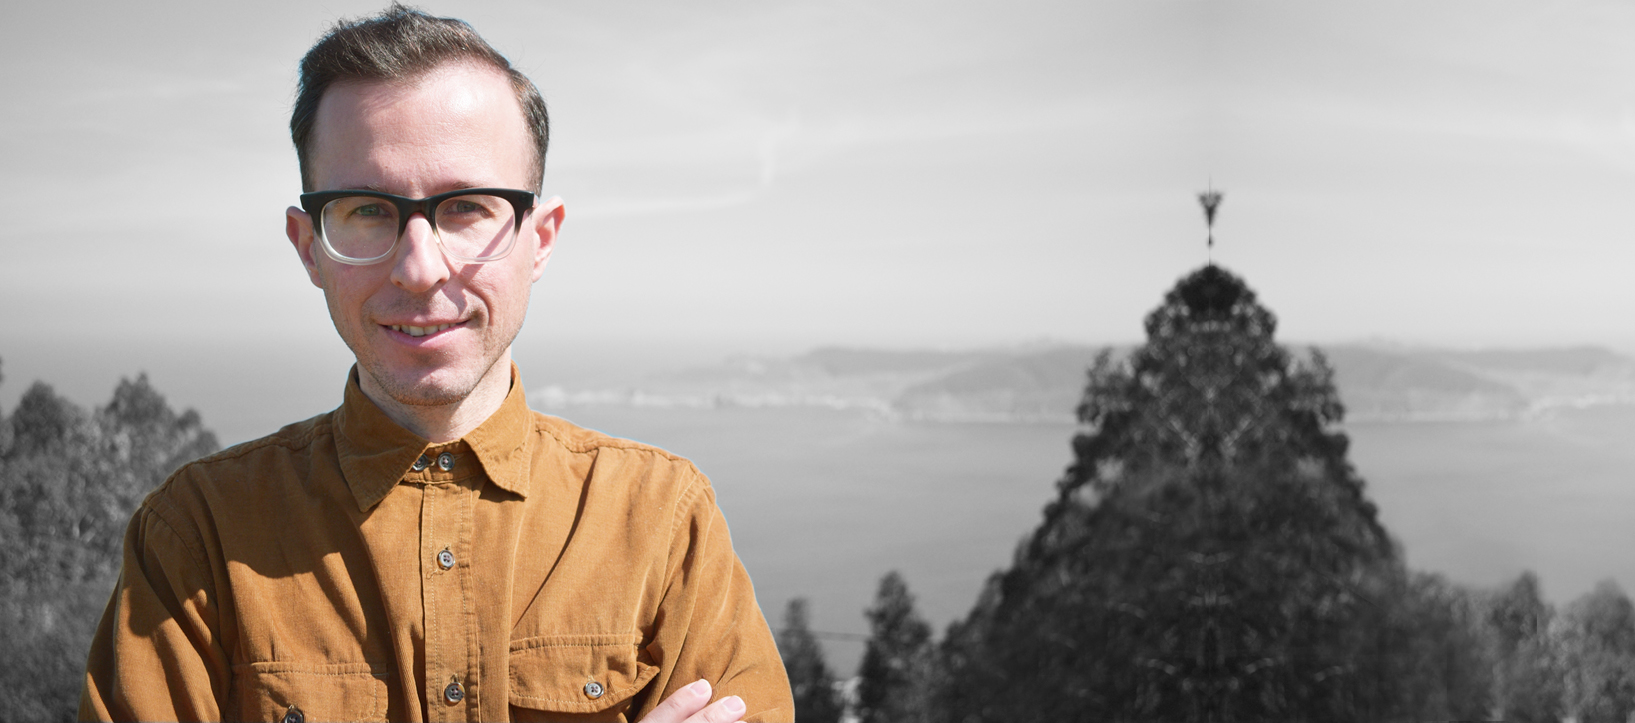
\includegraphics[trim=0 30 0 10, clip, width=\linewidth]{header-mountain.jpg} % Galicia

\includegraphics[trim=20 25 0 98, clip, width=1.3\linewidth]{header-flatiron.jpg} % Flatiron NY


%---------------------------------------------------------------------------------------
%	INTRODUCTION
%----------------------------------------------------------------------------------------
\transparent{0.85}%
\vspace{-100pt}
\hspace{0.4\linewidth}
\colorbox{introcolor}{
	\parbox{0.5\linewidth}{
		\transparent{1}%
		\begin{center}
		\larrow{sectcol}\textcolor{white}{
		  Enthusiast about Functional Programming, software engineering/craftsmanship, clean code, architectural/design patterns and programming languages theory.
		}
		\end{center}
	}
}
\vspace{28pt}

%============================================================================%
%
%	CV SECTIONS AND EVENTS (MAIN CONTENT)
%
%============================================================================%

%---------------------------------------------------------------------------------------
%	SUMMARY
%----------------------------------------------------------------------------------------
\cvsection{Summary}

[ \textcolor{gray}{\emph{Read the full detailed CV at}} \href{https://cv.gerardbosch.xyz}{https://cv.gerardbosch.xyz} ] \\[-2pt]

My background is mostly about designing/implementing backend systems and APIs. I have good analysis skills and can break down requirements well and transform that into code. Really concerned about the code itself, its readability, expressiveness and conciseness. Continuous improvement advocate and continuous refactor and code reuse as a mantra. Accidental-complexity fighter. Proactive and self-taught. Like learning~\emoji{smiley}, love crafting \emoji{heart}.

\vspace{12pt}

%---------------------------------------------------------------------------------------
%	EXPERIENCE
%----------------------------------------------------------------------------------------
\cvsection{Experience}

% Original cvevent example
%\cvevent{2020 - now}{}{}{}{}
%\textcolor{softcol}{\hrule}

% New custom commands below :)

\textbf{~~Presentations} \\[-2ex] \textcolor{softcol}{\hrule}\vspace{6pt}
\begin{tabular}{cl}
    2020 & \href{https://bit.ly/fp-short-intro}{Functional Programming super-short intro} \\
    2018 & \href{https://blockchain-presentation.gerardbosch.xyz}{A technical introduction to Blockchain technology} \\
\end{tabular}\vspace{5pt}


\cvposition{2021}{Software Engineer}{N26 Bank}

\cventry{
  Joined the fees team, which is in charge of designing and operating a new fee platform intended to be the new-standardized way of charging company-wide banking fees. That implied not only the creation of a dedicated microservice, also re-purposing and refactoring of existent ones (by DDD/CleanArch), along with APIs, as well as DB migrations.
}
\null
\cventry{
  Being a bank, testing is one of the most important and cared matters (pyramid testing, contract testing, regression, TDD,\ldots).
}
\null
\cventry{Stack: \textit{Kotlin, Spring Boot, Microservices, EDA, Kafka, REST, Postgres, Datadog, ELK, AWS,\ldots}}


\cvposition{2016 - 2021}{Senior Software Engineer}{GFT IT Consulting}
% ~~PROJECT HIGHLIGHTS (most relevant ones):

\cventry{
  \textit{Banc Sabadell}: \textbf{Middleware Architecture} (2020--2021) -- Redefine from scratch a whole new framework and development environment based on MsA, Spring Boot, API-First, Event Driven, DDD, Hexagonal and so forth -- \textbf{Role}: Software Engineer.
}
\null
\cventry{
  \textit{Banc Sabadell}: \textbf{PSD2 \& APIfication} (2018--2020) -- Design \& implement the APIs for the European regulatory PSD2 project, leading the first approach to API exposition for the Bank. Define and implement architectural components for the MsA where I was established as the technical lead for the dev team -- \textbf{Role}: Tech Lead.
}
\null
\cventry{
  \textit{Bankinter}: \textbf{Microservice Architecture} (2017) -- Development of an architecture based on MsA and Spring, providing the pre-configured components: from security, tracing, audit, error handling to cryptography; enabling developers to easily get started.
}

\vspace{5pt}
\cvposition{2014--2016}{Software Engineer}{ICG Software}
\cventry{Develop mobile solutions for retail in Android and Windows Phone platforms.}


\cvposition{2011--2013}{Researcher/developer}{AI Research Institute IIIA-CSIC}
%~~Spanish National Research Council. Innpacto-2011 (Spanish Science and Innovation Ministry),\par\vspace{2pt}
~~\emph{NEWMATICA: Intelligent and Energy Efficient Advanced System for Vacuum Waste Collection}.\\[3pt]
\cventry{Research Machine Learning algorithms based on \emph{Approximate Dynamic Programming}.}\\[-6pt]
\cventry{Implement a waste collecting simulator to optimize operational plans, run simulations, collect data/process results.}


%---------------------------------------------------------------------------------------
%	EDUCATION SECTION
%--------------------------------------------------------------------------------------
\cvsection{Education ~\lowercase{\emph{(to see more, view the \href{https://cv.gerardbosch.xyz}{\color{magenta}{CV version}})}}}

\vspace{-5pt}
\cvposition{2011}{M.Sc. Open Source Software Eng.}{University of Lleida}
\cventry{Master Thesis: \emph{Setting up and deployment of Sauron system for DNS system management at University of Lleida}. Mobility internship program at \emph{VIA UC}, Denmark.}

% \cvposition{2010}{Bachelor Computer Science}{University of Lleida}\vspace{-2pt}
% \cventry{Bachelor Thesis: \emph{Implementation of Golay codes in Sage Math.}}


\end{minipage}}%
\fcolorbox{white}{sidecolor}{\begin{minipage}[b][0.966\textheight][t]{0.33\linewidth}


%----------------------------------------------------------------------------------------
%	SIDE BAR
%----------------------------------------------------------------------------------------

\begin{metasection}{Contact}

	\icontext{MapMarker}{12}{Barcelona, Spain}{white}\\[5pt]
	%\icontext{MobilePhone}{12}{}{white}\\[5pt]
	\iconemail{Envelope}{12}{gerard.bosch@gmail.com}{gerard.bosch@gmail.com}{white} \\[5pt]
	\iconhref{Linkedin}{12}{linkedin.com/in/gerard-bosch}{https://www.linkedin.com/in/gerard-bosch}{white} \\[5pt]
	%\iconhref{MousePointer}{12}{Webpage}{Webpage}{white} \\[5pt]
	\iconhref{GithubAlt}{12}{github.com/gerardbosch}{https://github.com/gerardbosch}{white} \\[5pt]
	%\iconhref{StackOverflow}{12}{stackoverflow.com/users/6108874/gerard-bosch}{https://stackoverflow.com/users/6108874/gerard-bosch}{white} \\[5pt]
	%\iconhref{Twitter}{12}{@user}{https://twitter.com/user}{white} \\[5pt]

\end{metasection}

\vspace{-0.3cm}
\begin{metasection}{Programming Lang}\color{white}
\vspace{5pt}
\begin{tabular}{rl}

Java 17 &
\icon{Star}{12}{complcol}\icon{Star}{12}{complcol}\icon{Star}{12}{complcol}\icon{Star}{12}{complcol}\icon{Star}{12}{complcol} \\[2pt]

Scala 3 &
\icon{Star}{12}{complcol}\icon{Star}{12}{complcol}\icon{Star}{12}{complcol}\icon{Star}{12}{white}\icon{Star}{12}{white} \\[2pt]

Kotlin &
\icon{Star}{12}{complcol}\icon{Star}{12}{complcol}\icon{Star}{12}{complcol}\icon{Star}{12}{complcol}\icon{Star}{12}{white} \\[2pt]

Bash &
\icon{Star}{12}{complcol}\icon{Star}{12}{complcol}\icon{Star}{12}{complcol}\icon{Star}{12}{complcol}\icon{Star}{12}{white} \\[2pt]

Haskell &
\icon{Star}{12}{complcol}\icon{Star}{12}{complcol}\icon{Star}{12}{white}\icon{Star}{12}{white}\icon{Star}{12}{white} \\[2pt]

Python &
\icon{Star}{12}{complcol}\icon{Star}{12}{complcol}\icon{Star}{12}{complcol}\icon{Star}{12}{white}\icon{Star}{12}{white} \\[2pt]

Perl &
\icon{Star}{12}{complcol}\icon{Star}{12}{white}\icon{Star}{12}{white}\icon{Star}{12}{white}\icon{Star}{12}{white}

\end{tabular}
\end{metasection}


\vspace{-0.3cm}
\begin{metasection}{Technologies}

% \color{white}{\faDatabase~SQL} % alternative way, produces better vertical alignment than the custom \icontext
\icontext{Code}{12}{Spring Boot}{white}
\icontext{Code}{12}{Vavr}{white}
\icontext{Key}{12}{oAuth/JWT}{white} \\[5pt]

\icontext{Gavel}{12}{Maven/Gradle/sbt}{white}
\icontext{LifeSaver}{12}{JGitVer}{white} \\[5pt]

\icontext{Database}{12}{SQL}{white}
\icontext{PuzzlePiece}{12}{API First \& OpenAPI 3}{white} \\[5pt]

\icontext{Cube}{12}{Docker}{white}
\icontext{Cubes}{12}{OpenShift}{white}
\icontext{Cloud}{12}{Cloudflare}{white}

\end{metasection}


\vspace{-0.3cm}
\begin{metasection}{Tools}

\icontext{Code}{12}{IntelliJ / VSCode / vim :)}{white} \\[5pt]
\icontext{CodeFork}{12}{Git}{white} \icontext{Terminal}{12}{ZSH}{white} \icontext{Commenting}{12}{Codestream}{white}

\end{metasection}

% \begin{metasection}{Activities}
%
% \textcolor{white}{\LARGE{\icon{Gamepad}{24}{white} \icon{Headphones}{24}{white}  \icon{Bicycle}{24}{white}}}
% \end{metasection}
%
% \begin{metasection}{Operating Systems}
%
% \textcolor{white}{\LARGE{\icon{Linux}{24}{white} \icon{Apple}{24}{white}  \icon{Windows}{24}{white}}}
%
% \end{metasection}


%---------------------------------------------------------------------------------------
%	Knowledge Areas
%----------------------------------------------------------------------------------------

\vspace{-0.3cm}
\begin{metasection}{In graphics...}
\begin{center}

\smartdiagramset{
    bubble center node font = \footnotesize,
    bubble node font = \footnotesize,
    % specifies the minimum size of the bubble center node
    bubble center node size = 0.1cm,
    %  specifies the minimum size of the bubbles
    bubble node size = 0.9cm,
    % specifies which is the distance among the bubble center node and the other bubbles
    distance center/other bubbles = 0.5cm,
    % sets the distance from the text to the border of the bubble center node
    %distance text center bubble = 0.5cm,
    % set center bubble color
    bubble center node color = pastelblue,
    % define the list of colors usable in the diagram
    %set color list = {lightgray, materialcyan, orange, green, materialorange, materialteal, materialamber, materialindigo, materialgreen, materiallime},
    % sets the opacity at which the bubbles are shown
    %bubble fill opacity = 0.6,
    % sets the opacity at which the bubble text is shown
    %bubble text opacity = 1,
}
\smartdiagram[bubble diagram]{
    Knowledge \\ Areas,
    \normalsize{\textbf{Functional}} \\ \normalsize{\textbf{Programming}},
    DevOps,
    Reactive \\ Programming,
    \normalsize{\textbf{API design}} \\ \normalsize{\textbf{\& Tooling}},
    \normalsize{\textbf{~~Design~~}} \\ \normalsize{\textbf{patterns}},
    \textbf{Architectural} \\ \textbf{patterns},
    API\\ security
}

\vspace{2ex}
\smartdiagramset{
    bubble center node font = \footnotesize,
    bubble node font = \footnotesize,
    % specifies the minimum size of the bubble center node
    bubble center node size = 0.1cm,
    %  specifies the minimum size of the bubbles
    bubble node size = 0.9cm,
    % specifies which is the distance among the bubble center node and the other bubbles
    distance center/other bubbles = 0.5cm,
    % sets the distance from the text to the border of the bubble center node
    %distance text center bubble = 0.5cm,
    % set center bubble color
    bubble center node color = orange,
    % define the list of colors usable in the diagram
    %set color list = {lightgray, materialcyan, orange, green, materialorange, materialteal, materialamber, materialindigo, materialgreen, materiallime},
    % sets the opacity at which the bubbles are shown
    %bubble fill opacity = 0.6,
    % sets the opacity at which the bubble text is shown
    %bubble text opacity = 1,
}
\smartdiagram[bubble diagram]{
    \normalsize{Interest} \\ \normalsize{Areas},
    \textbf{~~~~DLTs \&~~~~} \\ \textbf{Blockchain},
    \textbf{Functional} \\ \textbf{Programming},
    \textbf{Artificial} \\ \textbf{Intelligence},
    \textbf{Big/Fast Data} \\ \textbf{\& Streaming}
}

\end{center}
\end{metasection}


%%%%%%%%%%%%%%%%%%%%%%%%%%%%%%%%%
\end{minipage}}    % end side bar
%%%%%%%%%%%%%%%%%%%%%%%%%%%%%%%%%

% Fork me on GitHub
% \scalebox{.9}{\forkme}
\forkme

%-------------------------------------------------------------------------------------------------
%	ARTIFICIAL FOOTER (fancy footer cannot exceed linewidth)
%--------------------------------------------------------------------------------------------------

\vspace{-4pt}
\hspace{-0.25\linewidth}\colorbox{bgcol}{\makebox[1.5\linewidth][c]{
  \mystrut \small \textcolor{white}{
    ~~~\LaTeX~source of this \textit{résumé} is available at
    {\normalsize\faGithub}~\href{https://github.com/gerardbosch/resume}{\color{white}{github.com/gerardbosch/resume}}
    ~$\cdot$~
    Built/Delivered by GH Actions/Cloudflare
    ~$\cdot$~
    Last updated: \today
  }
}}

%============================================================================%
%
%	DOCUMENT END
%
%============================================================================%
\end{document}
